% # minted require -shell-escape to run  external script.
% # -8bit avoid ^^I for tabs in minted.
% $ xelatex -shell-escape -8bit main
% # If any change in the bibliography
% $ biber main
% # If any change with the abbreviation or acronym
% $ makeglossaries main
% #Then compile again
% $ xelatex -shell-escape -8bit main
% #And if still some citation or label warnings, compile once more
% $ xelatex -shell-escape -8bit main

%----------------------------------------------------------------------------------------
%	THESIS INFO
%----------------------------------------------------------------------------------------

% All general information (main language, title, author (you), degree programme, major
% option, etc.)
% Edit the file chapters/0info.tex to change these information
\documentclass[12pt,a4paper,oneside,article]{memoir}%Do not touch this first line ;)

% Global information (title of your thesis, your name, degree programme, major, etc.)

%\def\bilingual{yes}%For Finnish students, you must have 2 abstracts, one in English and one in your native language (Finnish or Swedish), so "yes", your thesis is bilingual.
\def\bilingual{yes}%For international student writing in English, only one language and one abstract.

%\def\thesislang{finnish} %change this depending on the main language of the thesis.
\def\thesislang{english} % "english" is the only other supported language currently. If someone has the swedish, please contribute!

%\def\secondlang{english} %if the main language is Finnish (or Swedish), you must have 2 abstracts (one in Finnish (or Swedish) and one in English)
%\def\secondlang{finnish}
%If the main language is English and that you are native Finnish (or Swedish) speaker, you must have also abstract in your native language on top of the English one.

\author{Nicolas Kyejo}

%\def\alaotsikko{Alaotsikko/Subtitle} %DISABLED, seems not to be an option with the 2018 template. If you really need it, uncomment and modify style/title.tex accordingly.

%License
%When publishing your thesis to theseus.fi, you can keep all rights reserved to you,
%or use one of the Creative Commons https://creativecommons.org/licenses/?lang=en
%This attribute will set the license in the metadata of the generated pdf.
%possible options (case sensitive):
%all (keep all rights reserved to yourself)
%by (Attribution)
%by-sa (Attribution-ShareAlike)
%by-nd (Attribution-NoDerivs)
%by-nc (Attribution-NonCommercial)
%by-nc-sa (Attribution-NonCommercial-ShareAlike)
%by-nc-nd (Attribution-NonCommercial-NoDerivs)
%Note that theseus do not accept dedication to public domain CC0
\def\thesiscopy{by-sa}

%Finnish section, for title/abstract
\def\otsikko{Haitallisen verkkoliikenteen rikosteknisen analyysijärjestelmän toteuttaminen}
\def\tutkinto{Insinööri (AMK)}
\def\kohjelma{Tieto- ja viestintätekniikka}
\def\suuntautumis{IoT ja Pilvipalvelut}
\def\thesisfi{Insinöörityö}
\def\ohjaajat{
Janne Salonen, Osaamisaluepäällikkö, ICT ja tuotantotalous
}
\def\tiivistelma{
    Insinöörityön päätavoitteena oli koneoppimismallien luominen pahantahtoisen verkkoliikenteen havaitsemiseksi. Nämä mallit luotiin käyttäen `K-nearest Neighbors'-, `Logistic Regression'-, `Random Forest'-, ja `Multi-Layer Perceptron' -algoritmeja. Mallien koulutuksessa käytetty datasetti oli CICIDS2017-datasetti. Lopullisessa arviointivaiheessa virtuaalisessa lähiverkossa kaapattua liikennettä käytettiin mallien arvioimiseen. \newline

    Mallien suorituskyky ja ennusteet viittasivat siihen, että niitä voitaisiin käyttää tehokkaasti verkkorikostekniikassa kyberhyökkäysten tunnistamiseksi. Insinöörityö osoitti, että tällainen toteutettu järjestelmä oli erittäin riippuvainen avoimien datasettien saatavuudesta, joten vaiva näyttää olevan perusteltua, jos laadukkaita avoimia datasetteja on saatavilla ja käytössä.

}
\def\avainsanat{tunkeutumisen tunnistusjärjestelmä, koneoppiminen, kyberturvallisuus}
\def\aihe{Kehitys ja arviointi edullisen verkkotutkintajärjestelmän toteuttamiseksi pahantahtoisen verkkoliikenteen havaitsemiseksi.}

\title{Implementation of a forensic analysis system for malicious network traffic}
\def\metropoliadegree{Bachelor of Engineering}
\def\metropoliadegreeprogramme{Information and Communication Technology}
\def\metropoliaspecialisation{IoT and Cloud Computing}
\def\thesisen{Bachelor’s Thesis}
\def\metropoliainstructors{
Janne Salonen, Head of School (ICT)
}
\def\abstract{
    The objective of this thesis was to develop and evaluate a forensic system for detecting malicious network traffic, focusing on its practical implementation and effectiveness as a low-cost security solution. To support this goal, only open and freely available tools were used. \newline

    The main solution used in the thesis project was the creation of machine learning models to detect malicious network traffic. These models were created from K-nearest Neighbors, Logistic Regression, Random Forest, and Multi-Layer Perceptron algorithms. The dataset used in the training of the models was the CICIDS2017 dataset. As a final evaluation step, traffic captured in a virtual LAN was used the assess the models. \newline

    The performance and predictions of the models indicated that they could be used effectively in a network forensic system for identifying cyberattacks.
    The thesis showed that such an implemented system was profoundly reliant on the availability of open datasets, hence the cost in terms of effort seems to be justified if quality and open datasets are available and used.

}
\def\metropoliakeywords{network forensics, packets, intrusion detection, machine-learning, cybersecurity}
\def\subject{Development and evaluation of a low-cost forensic system for detecting malicious network traffic}


%----------------------------------------------------------------------------------------
%	GLOBAL STYLES
%----------------------------------------------------------------------------------------

% If you need extra package, etc. modify the style/style.tex file.
% If you are using Windows OS, you will need to change default font to Arial in that
% style/style.tex file (or install Liberation Sans font to your system).
% If you are using MacOS or linux, make sure you have Liberation Sans font installed.
% Global style. Normally should not be edited.
% If you use windows OS, eventually change \setmainfont to Arial
% Check around commit https://github.com/panunu/metropolia-thesis-latex/commit/a0c15ac77bab1a52c59c517a18080938e57bf5ef
% to see how the font files were manually added (after downloading them: https://pagure.io/liberation-fonts/ )

%\usepackage[l2tabu, orthodox]{nag}%check for obsolete packages (with outdated nag package?)

%condition e.g. for adding or not space in TOC,...
\usepackage{etoolbox}
\ifdefstring{\bilingual}{yes}{
  \usepackage[\secondlang,\thesislang]{babel}% finnish (or swedish) and english
}{
  \usepackage[\thesislang]{babel}% english only
}
\usepackage{iflang}
\usepackage{amsmath}
\usepackage{amsfonts}%extra mathematical symbols
\usepackage{amssymb}
\usepackage{fontspec}
\usepackage{titlesec}
\usepackage{mathtools}%enhance the appearance of documents containing a lot of mathematics
\usepackage[amssymb]{SIunits}
\usepackage[version=3]{mhchem}
\usepackage{tikz} % mindmaps, flowcharts, piecharts, examples at http://www.texample.net/tikz/examples/
\usetikzlibrary{shapes.geometric, arrows}

\usepackage{ragged2e}
\IfLanguageName{finnish}{
  \RaggedRight%2021 template, align left and hyphennization for Finnish version
  \setlength{\RaggedRightRightskip}{0pt plus 1fil}%TODO: fix the Overfull/Underfull warnings when \RaggedRight (likely in title and abstact)
}{}
\makeatletter
  \let\@gnewline\@raggedtwoe@saved@gnewline% Restore original functionality of \newline
  \let\\\@raggedtwoe@savedcr% Restore original functionality of \\
\makeatother

%for compact list
\usepackage{enumitem}
%\usepackage{verbatim}%for block comment
%forcing single line spacing in bibliography
\DisemulatePackage{setspace}
\usepackage{setspace}
%\usepackage{eurosym}%euro symbol
%try to count
\usepackage{totcount}
%insert source code
%require -8bit -shell-escape in the xelatex compile command
%if compiling locally, consider options cachedir=minted,outputdir=~/.tex
\usepackage[newfloat,outputdir=out/]{minted}
\setminted{tabsize=2,linenos,breaklines,breaksymbolleft={\quad},baselinestretch=1}
\setmintedinline{breaklines,breakanywhere}
\usepackage[singlelinecheck=false]{caption}
%force the width of a table instead of column
\usepackage{tabularx}
\usepackage{booktabs} %why not booktabs? :3

\usepackage{csquotes}% avoid warning with babel

\usepackage{float} % For forced figure location with modifier H (\begin{figure}[H])
\usepackage{wrapfig}

% citep-macro for reference with period inside square brackets [1.]
\newcommand{\citep}[1]{
 \renewcommand\citeright{.]}
 \cite{#1}
 \renewcommand\citeright{]}
}

%set date format to D.M.YYYY
\def\pvm{\the\day.\the\month.\the\year}
%set date format to D Month YYYY
\usepackage[en,useregional=false]{datetime2}
\DTMsetup{datesep=.}
\DTMnewdatestyle{dMonthyyyy}
{%
  \renewcommand{\DTMdisplaydate}[4]{%
    \number##3 % day
    ~% separator
    \DTMenglishmonthname{##2}% month name
    ~% separator
    \number##1% year
  }%
  \renewcommand{\DTMDisplaydate}[4]{%
    \DTMdisplaydate{##4}{##3}{##2}{##1}%
  }%
}
\DTMsetdatestyle{dMonthyyyy}
\date{\today}

\newcommand\tn[1]{\textnormal{#1}} %use \tn instead of \textnormal
\newcommand\reaction[1]{\begin{equation}\ce{#1}\end{equation}} %\reaction{} for chemical reactions

%NORMAL TEXT
%all text, title, etc. in the same font: Arial
%NOTE: fontname is case-sensitive
%\setmainfont[Scale=0.98]{Liberation Sans}
\setmainfont[Scale=0.98]{Arial}
%line space
\linespread{1.46}
\AtBeginEnvironment{tabular}{\singlespacing}
%\doublespacing
%margin
%geometry moved after hyperref
\setlength{\parindent}{0pt} %first line of paragraph not indented
\setlength{\parskip}{16.5pt} %one empty line to separate paragraph
%list with small line space separation
\tightlists
\setlist[itemize]{before=\singlespacing,itemsep=6pt,leftmargin=63pt,labelsep=22pt,topsep=1.5pt,partopsep=0pt,after=\vspace{-22pt}\newline}
\setlist[enumerate]{before=\singlespacing,itemsep=6pt,leftmargin=63pt,labelsep=22pt,topsep=1.5pt,partopsep=0pt,after=\vspace{-22pt}\newline}

%IMAGE - FIGURE
%the figures should be placed in the "illustration" folder
\graphicspath{{illustration/}}
\usepackage{svg}
%figure number without chapter (1.1, 1.2, 2.1) to (1, 2, 3)
\counterwithout{figure}{chapter}
%border around images
\setlength\fboxsep{0pt}
\setlength\fboxrule{0.5pt}
%space after figure caption (and other float elements)
\setlength{\belowcaptionskip}{-7pt}
\setlength{\intextsep}{16.5pt}%space around floats
\AtBeginEnvironment{table}{\addvspace{16.5pt}}

%TABLE
\counterwithout{table}{chapter}

%SOURCE CODE
\newenvironment{code}{\captionsetup{type=listing}}{}
\IfLanguageName{finnish}{\SetupFloatingEnvironment{listing}{name=Koodiesimerkki}}{}%was Listaus
%\counterwithout{lstlisting}{chapter}
%moved after begin document, otherwise does not compile

%TOC
%change toc title
\IfLanguageName{finnish}{\addto{\captionsfinnish}{\renewcommand*{\contentsname}{Sisällys}}}{}
%remove dots
\renewcommand*{\cftdotsep}{\cftnodots}
%chapter title and page number not in bold
\renewcommand{\cftchapterfont}{\normalfont}
\renewcommand{\cftchapterpagefont}{\normalfont}
%sub section in toc
\setcounter{tocdepth}{2}
%subsection numbered
\setcounter{secnumdepth}{2}
\renewcommand{\tocheadstart}{\vspace*{-33.5pt}}
\renewcommand{\printtoctitle}[1]{\fontsize{13.5pt}{13.5pt}\bfseries #1\vspace*{-4pt}}
%\renewcommand{\aftertoctitle}{\vspace*{-22pt}\afterchaptertitle}
%spacing after a chapter in toc
\preto\section{%
  \ifnum\value{section}=0\addtocontents{toc}{\vskip11pt}\fi
}
%spacing after a section in toc
\renewcommand{\cftsectionaftersnumb}{\vspace*{-3pt}}
%spacing after a subsection in toc
\renewcommand{\cftsubsectionaftersnumb}{\vspace*{-1pt}}
%appendix in toc with "Appendix " + num
\IfLanguageName{finnish}{
  \renewcommand*{\cftappendixname}{Liite\space}
  \renewcommand{\appendixtocname}{Liitteet}
}{\renewcommand*{\cftappendixname}{Appendix\space}}
%appendix header
\IfLanguageName{finnish}{\def\appname{Liite\space}}{\def\appname{Appendix\space}}

%TITLES
%chapter title
%\clearforchapter{\clearpage}
\titleformat{\chapter}
{\fontsize{14pt}{14pt}\bfseries\linespread{1}}%\clearpage
{\thechapter}{.5cm}{}
\titlespacing*{\chapter}{0pt}{-.42cm}{.5pt}
\titleformat{\section}
{\fontsize{13.5pt}{13.5pt}\normalfont}
{\thesection}{.5cm}{}
\titlespacing*{\section}{0pt}{9pt}{0pt}
\titleformat{\subsection}
{\fontsize{12.7pt}{12.7pt}\normalfont}
{\thesubsection}{.5cm}{}
\titlespacing*{\subsection}{0pt}{11pt}{0pt}


%QUOTE
\renewenvironment{quote}
{\list{}{\rightmargin=0pt\leftmargin=2.2cm\topsep=-14pt}%
  \item\relax\singlespacing}%\fontsize{10pt}{10pt}
    {\vspace{8pt}\endlist}

%BIBLIOGRAPHY
\usepackage[
backend=biber,
bibencoding=utf8,%
citetracker=true,%
isbn=false,%
doi=false,%
url=true,%
usetranslator=true,%
bibstyle=ext-authoryear,%
citestyle=numeric-comp,%
sorting=none,%
sortcites=true,%
block=none,%
terseinits=false,%
giveninits=false,%
maxbibnames=99,%
]{biblatex}

% I needed to format the date in the bibliography
\renewbibmacro*{urldate}{
    \printtext{Accessed on}
    \DTMdisplaydate{\thefield{urlyear}}{\thefield{urlmonth}}{\thefield{urlday}}{-1}
}

\setlength{\bibitemsep}{11pt}
\setlength{\biblabelsep}{1cm}%with 1cm horizontal gap

\makeatletter
\RequireBibliographyStyle{numeric}
\makeatother

% set right format
\renewcommand*{\multicitedelim}{;\space}
\renewcommand*{\multinamedelim}{;\space}
\renewcommand*{\finalnamedelim}{~\&\space}
\DeclareFieldFormat{biblabeldate}{#1}
\DeclareDelimFormat[bib]{nameyeardelim}{\addperiod\space}
%\DeclareNameAlias{sortname}{last-first} % deprecated
\DeclareNameAlias{default}{family-given}
\DeclareFieldFormat{labelnumberwidth}{#1} % remove () from label number
\DeclareFieldFormat{title}{#1} % normal font for title
\DeclareFieldFormat{citetitle}{#1}
\DeclareFieldFormat{journaltitle}{#1} % remove underline
\DeclareFieldFormat*{url}{%
\ifentrytype{online}{\IfLanguageName{finnish}{Verkkoaineisto}{Online}\addperiod\space}{}%
\ifentrytype{video}{Video\addperiod\space}{}%
\textless\url{#1}\textgreater\addperiod
} % you can modify how to url looks here
%TODO: remove leading 0 for day and month for Finnish dates
\DeclareFieldFormat{urldate}{\space\bibstring{urlseen}\space#1} % remove () from date
%try set translation to biblio
\DefineBibliographyStrings{english}{%
    urlfrom = {available at},%
    urlseen = {Visited on},%
    fromenglish = {from English},%
    fromfinnish = {from Finnish},%
    fromgerman = {from German},%
    fromjapanese = {from Japanese},%
}
\DefineBibliographyStrings{finnish}{%
  %  urlfrom={Linkki: },%
    urlfrom = {},%
    urlseen = {Luettu},%
    fromjapanese = {japanista},%
    fromenglish = {englannista},%
    fromfinnish = {suomesta},%
    fromgerman = {saksasta},%
}
{
  %new cite command: "Vancouver Short"
  \DeclareCiteCommand{\citeVS}
    {\usebibmacro{prenote}}
    {\usebibmacro{author}, \usebibmacro{title}}
    {\multicitedelim}
    {\usebibmacro{postnote}}

  % new cite command: "Vancouver Short Collection" - necessary when referencing whole collections.
  \DeclareCiteCommand{\citeVSc}
    {\usebibmacro{prenote}}
    {\usebibmacro{editor}, \usebibmacro{title}}
    {\multicitedelim}
    {\usebibmacro{postnote}}
}

% when citing multiple sentences/entire paragraph, add a dot inside the brackets
\DeclareCiteCommand{\citep}[\mkbibbrackets]
  {\usebibmacro{cite:init}%
    \usebibmacro{prenote}}
  {\usebibmacro{citeindex}%
     \usebibmacro{cite:comp}}
  {\multicitedelim}
  {\usebibmacro{postnote}\addperiod}

\addbibresource{biblio.bib}% for biblatex you need out \printbibliography too

%count the appendices (since the chapter counter is reset after \appendix).
%! require to complie 2 times
\regtotcounter{chapter}

% metadata (title, author, lang,...) for accessibility, etc.
\usepackage{hyperref}
\usepackage{hyperxmp}
\def\isolang{\IfLanguageName{finnish}{fi}{en}} %iso code (based on main language)
\ifdefstring{\thesiscopy}{all}{%
    \def\copyen{Copyright \textcopyright\ \the\year{}, \theauthor}
    \def\copyfi{Kaikki oikeudet pidätetään.  \textcopyright\ \the\year{}, \theauthor}
  }{%
    \usepackage[type={CC},modifier={\thesiscopy},version={4.0},]{doclicense}
    \def\copyen{\thetitle\ \textcopyright\ \the\year{} by \theauthor\ is licensed under \doclicenseLongNameRef}
    \def\copyfi{\otsikko\ \textcopyright\ \the\year{}, jonka tekijä on \theauthor, on lisensoitu \doclicenseLongNameRef}
}
\hypersetup{%
  pdfdisplaydoctitle,
  %breaklinks=true,%searching for overfull warnings
  pdfencoding=auto,
  bookmarksdepth=subsection,
  unicode=true,
  keeppdfinfo=true,
  pdflang={\isolang},
  pdfmetalang={\isolang},
  pdftitle={\IfLanguageName{finnish}{\otsikko}{\thetitle}},
  pdfkeywords={\IfLanguageName{finnish}{\avainsanat}{\metropoliakeywords}},
  pdfcopyright={\IfLanguageName{finnish}{\copyfi}{\copyen}},
  pdfsubject={\IfLanguageName{finnish}{\aihe}{\subject}},
}

\ifdefstring{\bilingual}{yes}{%metadata (title and copyright) in multiple language
  \XMPLangAlt{\IfLanguageName{finnish}{en}{fi}}{%
    pdftitle={\IfLanguageName{finnish}{\thetitle}{\otsikko}},
    pdfcopyright={\IfLanguageName{finnish}{\copyen}{\copyfi}},
    pdfsubject={\IfLanguageName{finnish}{\subject}{\aihe}},
  }
}{}
\urlstyle{same}

%moved after hyperred as can cause conflicts
\usepackage{pdfcomment}%try the alt text for graphics
\usepackage{accsupp}
\newcommand{\AltText}[2]{\BeginAccSupp{method=pdfstringdef,unicode,Alt={{#1}}}\pdftooltip{{#2}}{{#1}}\EndAccSupp{}}

\usepackage[top=2.5cm, bottom=3cm, left=4cm, right=2cm, nofoot]{geometry}

\usepackage{pgfplots} %simple plots etc
\pgfplotsset{compat=1.16}
\usepackage{pgfplotstable}

% Abbreviations, acronym and glossary, in case of bug, remove temporary the noredefwarn
\usepackage[acronym,toc,nonumberlist,section=chapter,noredefwarn]{glossaries}%xindy,%toc, ,nomain
\newglossarystyle{mystyle}{%
  \setglossarystyle{list}% base this style on the list style
  \renewcommand*{\glossentry}[2]{%
  \item[\glsentryitem{##1}%
    \glstarget{##1}{\glossentryname{##1}:}]
  \glossentrydesc{##1}\glspostdescription\space ##2}
}
\setglossarystyle{mystyle}

\renewcommand*{\glsclearpage}{}

% Normally, you do not need to modify the title style. It's content comes from the
% chapters/0info.tex file.
% TITLE PAGE
% Normally, you should not edit this file.

\makeatletter
\renewcommand{\maketitle}{
\newgeometry{left=4cm,top=2.7cm}
\thispagestyle{empty}

\AltText{\IfLanguageName{finnish}{Metropolia Ammattikorkeakoulu.}{Metropolia University of Applied Sciences.}}{\includegraphics[width=9.1cm,keepaspectratio]{Metropolia_L_oranssi}}

\IfLanguageName{finnish}{
\vspace*{1.36cm}
}{
\vspace*{1.18cm}
}
\tn{\large\theauthor\\[9.2mm]{\fontsize{27.5pt}{27.5pt}\normalfont\color[RGB]{155,50,35}\IfLanguageName{finnish}{\otsikko}{Implementation of a Forensic Analysis System for Malicious Network Traffic}}}%\\[22pt]\LARGE\alaotsikko\\[1.75cm]}

\vspace*{2.38cm}
{\setstretch{1.512}
\IfLanguageName{finnish}{
  Metropolia Ammattikorkeakoulu\\
  \tutkinto \\
  \kohjelma \\
  \thesisfi\\
  \pvm % D.M.YYYY date format for Finnish.
} {
  Metropolia University of Applied Sciences\\
  \metropoliadegree \\
  \metropoliadegreeprogramme \\
  \thesisen\\
  \@date %D Month YYYY for English
}
}
\clearpage
\restoregeometry
}
\makeatother



%----------------------------------------------------------------------------------------
%	ABBREVIATION AND GLOSSARY
%----------------------------------------------------------------------------------------

% Add/edit all your acronyms, abbreviations, glossary entries, etc. definitions in
% chapters/0abbr.tex file.
% You can have as many as you wish. Only the ones you use in your text (inserted with
% \gls{} command) will print in the Glossary/Lyhenteet.
% Generate the glossary
\makeglossaries

% Acronyms, abbreviations, etc.

\newacronym{sql}{SQL}{Structured Query Language}
\newacronym{DoS}{DoS}{Denial-of-Service}
\newacronym{DDoS}{DDoS}{Distributed Denial-of-Service}
\newacronym{siem}{SIEM}{Security Information and Event Management}
\newacronym{ids}{IDS}{Intrusion Detection System}
\newacronym{sids}{SIDS}{Signature-based Intrusion Detection System}
\newacronym{aids}{AIDS}{Anomaly-based Intrusion Detection System}
\newacronym{ips}{IPS}{Intrusion Prevention System}
\newacronym{icmp}{ICMP}{Internet Control Message Protocol}
\newacronym{xss}{XSS}{Cross-Site Scripting}
\newacronym{dom}{DOM}{Document Object Model}
\newacronym{lan}{LAN}{Local Area Network}
\newacronym{knn}{KNN}{K-nearest Neighbors}
\newacronym{mlp}{MLP}{Multi-Layer Perceptron}
\newacronym{ann}{ANN}{Artificial Neural Network}
\newacronym{dvwa}{DVWA}{Damn Vulnerable Web Application}
\newacronym{pcap}{PCAP}{Packet Capture}
\newacronym{gui}{GUI}{Graphical User Interface}
\newacronym{ssh}{SSH}{Secure Shell}
\newacronym{dns}{DNS}{Domain Name System}
\newacronym{ftp}{FTP}{File Transfer Protocol}
\newacronym{http}{HTTP}{Hypertext Transfer Protocol}



% Glossary entries

\newglossaryentry{zero-day}{
    name={zero-day},
    description={a type of vulnerability or flaw in software, hardware, or firmware known only to the attacker and not to the developers of the affected system, making it difficult to defend against}
}

\newglossaryentry{cv}{
    name={cross-validation},
    description={a method to test the accuracy of a machine learning model by splitting the dataset into smaller subsets, training the model on some subsets and testing it on the others. This process is repeated multiple times to ensure the model's performance is not overfitting and to estimate its generalization performance on new data}
}

\newglossaryentry{lr}{
    name={Linear Regression},
    description={a statistical method used to model the relationship between two variables by fitting a straight line through the data points to minimize the sum of squared residuals, with the goal of predicting the value of one variable (dependent variable) based on the value of another variable (independent variable)}
}

\newglossaryentry{train-data}{
name={train data},
description={a labeled dataset used to train a machine learning model}
}

\newglossaryentry{test-data}{
name={test data},
description={a separate and independent dataset that is used to evaluate the performance and generalization capability of a trained machine learning model}
}

\newglossaryentry{decision-threshold}{
name={decision threshold},
description={a probability value that is used to classify observations into one of two (or more) classes. If the predicted probability of an observation belonging to one class is above the decision threshold, it is classified as belonging to that class; otherwise, it is classified as belonging to the other class}
}

\newglossaryentry{ensemble-method}{
name={ensemble method},
description={a technique that combines the predictions of multiple learning algorithms to improve prediction}
}

\newglossaryentry{over-fitting}{
name={overfitting},
description={a situation where a trained model performs very well on the training data but fails to generalize to new, unseen data}
}

\newglossaryentry{false-negative}{
name={false-negative},
description={a missed positive prediction}
}

\newglossaryentry{false-positive}{
name={false-positive},
description={an incorrect classification of a negative prediction as positive, that is to say, noise}
}

\newglossaryentry{pr-mode}{
name={promiscuous mode},
description={a feature in packet capture where a network interface card captures all packets on a network, including those not addressed to it}
}

\newglossaryentry{feat-extr}{
name={feature extraction},
description={a process of selecting and transforming raw data into a set of meaningful features that can be used for model training and prediction}
}

\newglossaryentry{hyper-param}{
name={hyperparameters},
description={parameters set before training in a machine learning model and are not learned from the data.
They control the behavior of the learning algorithm and can significantly impact the performance of the trained model}
}


%----------------------------------------------------------------------------------------
%	DOCUMENT STARTS HERE...
%----------------------------------------------------------------------------------------

\begin{document}
\IfLanguageName{finnish}{
}{
  \raggedright%2021 template, align left, no hyphennization for English version
}
\counterwithout{listing}{chapter}

%----------------------------------------------------------------------------------------
%	TITLE PAGE
%----------------------------------------------------------------------------------------

\input{style/title_headers.tex}
\maketitle
\newpage

%----------------------------------------------------------------------------------------
%	ABSTRACT / Tiivistelmä
%----------------------------------------------------------------------------------------

% If you are international student writing in English, ignore the Finnish abstract.
% If you are Finnish citizen, you must have 2 abstracts, one in Finnish (or Swedish
% depending on your mother tongue) and one in English regardless of the main language of
% your thesis. Normally, you do not need to modify the abstract style. It's content comes
% from the chapters/0info.tex file.
\ifdefstring{\bilingual}{no}{%
    % Abstract in English
% Normally, you should not edit this file. Everything comes from chapter/0info.tex

\pagestyle{empty} %remove page number
\newgeometry{top=2.45cm,left=4cm,right=.5cm}
\begin{otherlanguage}{english}
{\large\textbf{Abstract}}
{\renewcommand{\arraystretch}{1.1}
  \begin{tabular}{@{}p{4.7cm} >{\raggedright\arraybackslash}p{10.8cm}@{}}
  Author: & \makeatletter\@author\makeatother
  \\
  Title: & \makeatletter\@title\makeatother
  \\
  Number of Pages: & \pageref*{LastPage} pages% + \total{chapter} appendices
  \\
  Date: & \makeatletter\thedate\makeatother
  \\[6.5mm]
  Degree: & \metropoliadegree
  \\
  Degree Programme: & \metropoliadegreeprogramme
  \\
  Professional Major: & \metropoliaspecialisation
  \\
  Supervisors: & \metropoliainstructors
  \\[6mm]
  \cmidrule[.7pt](l{-.15em}r{5.5em}){1-2}
  \\
  \multicolumn{2}{>{\raggedright}p{15.5cm}}{
    \abstract
  }
  \\
  \\
  Keywords: & \metropoliakeywords
  \\
\end{tabular}
}
\end{otherlanguage}
\restoregeometry
\clearpage


    }{%
    \IfLanguageName{finnish}{%order of abstracts based on main language and spacing hell
        % Abstract in Finnish
% Normally, you should not edit this file. Everything comes from chapter/0info.tex

\pagestyle{empty} %remove page number
\newgeometry{top=1.5cm,left=4cm,right=.5cm}
\begin{otherlanguage}{finnish}
{\large\textbf{Tiivistelmä}}
{\renewcommand{\arraystretch}{1.1}
  \begin{tabular}{@{}p{4.7cm} >{\raggedright\arraybackslash}p{10.8cm}@{}}
  Tekijä: & \makeatletter\@author\makeatother
  \\
  Otsikko: & \otsikko
  \\
  Sivumäärä: & \pageref*{LastPage} sivua% + \total{chapter} liitettä
  \\
  Aika: & \pvm
  \\[6.5mm]
  Tutkinto: & \tutkinto
  \\
  Tutkinto-ohjelma: & \kohjelma
  \\
  Ammatillinen pääaine: & \suuntautumis
  \\
  Ohjaajat: & \ohjaajat
  \\[11mm]
  \cmidrule[.7pt](l{-.15em}r{5.5em}){1-2}
  \multicolumn{2}{>{\raggedright}p{15.5cm}}{
  \vspace{.2mm}
  \tiivistelma
  }
  \\
  \\
  Avainsanat: & \avainsanat
  \\
\end{tabular}
}
\end{otherlanguage}
\restoregeometry
\clearpage


        % Abstract in English
% Normally, you should not edit this file. Everything comes from chapter/0info.tex

\pagestyle{empty} %remove page number
\newgeometry{top=1.77cm,left=4cm,right=.5cm}
\begin{otherlanguage}{english}
{\large\textbf{Abstract}}
{\renewcommand{\arraystretch}{1.1}
  \begin{tabular}{@{}p{4.7cm} >{\raggedright\arraybackslash}p{10.8cm}@{}}
  Author: & \makeatletter\@author\makeatother
  \\
  Title: & \makeatletter\@title\makeatother
  \\
  Number of Pages: & \pageref*{LastPage} pages% + \total{chapter} appendices
  \\
  Date: & \makeatletter\thedate\makeatother
  \\[6.5mm]
  Degree: & \metropoliadegree
  \\
  Degree Programme: & \metropoliadegreeprogramme
  \\
  Professional Major: & \metropoliaspecialisation
  \\
  Supervisors: & \metropoliainstructors
  \\[9mm]
  \cmidrule[.7pt](l{-.15em}r{5.5em}){1-2}
  \\
  \multicolumn{2}{>{\raggedright}p{15.5cm}}{
    \abstract
  }
  \\
  \\
  Keywords: & \metropoliakeywords
  \\
\end{tabular}
}
\end{otherlanguage}
\restoregeometry
\clearpage


        }{
        % Abstract in English
% Normally, you should not edit this file. Everything comes from chapter/0info.tex

\pagestyle{empty} %remove page number
\newgeometry{top=2.45cm,left=4cm,right=.5cm}
\begin{otherlanguage}{english}
{\large\textbf{Abstract}}
{\renewcommand{\arraystretch}{1.1}
  \begin{tabular}{@{}p{4.7cm} >{\raggedright\arraybackslash}p{10.8cm}@{}}
  Author: & \makeatletter\@author\makeatother
  \\
  Title: & \makeatletter\@title\makeatother
  \\
  Number of Pages: & \pageref*{LastPage} pages% + \total{chapter} appendices
  \\
  Date: & \makeatletter\thedate\makeatother
  \\[6.5mm]
  Degree: & \metropoliadegree
  \\
  Degree Programme: & \metropoliadegreeprogramme
  \\
  Professional Major: & \metropoliaspecialisation
  \\
  Supervisors: & \metropoliainstructors
  \\[6mm]
  \cmidrule[.7pt](l{-.15em}r{5.5em}){1-2}
  \\
  \multicolumn{2}{>{\raggedright}p{15.5cm}}{
    \abstract
  }
  \\
  \\
  Keywords: & \metropoliakeywords
  \\
\end{tabular}
}
\end{otherlanguage}
\restoregeometry
\clearpage


        % Abstract in Finnish
% Normally, you should not edit this file. Everything comes from chapter/0info.tex

\pagestyle{empty} %remove page number
\newgeometry{top=2.04cm,left=4cm,right=.5cm}
\begin{otherlanguage}{finnish}
{\large\textbf{Tiivistelmä}}
{\renewcommand{\arraystretch}{1.1}
  \begin{tabular}{@{}p{4.7cm} >{\raggedright\arraybackslash}p{10.8cm}@{}}
  Tekijä: & \makeatletter\@author\makeatother
  \\
  Otsikko: & \otsikko
  \\
  Sivumäärä: & \pageref*{LastPage} sivua% + \total{chapter} liitettä
  \\
  Aika: & \pvm
  \\[6.5mm]
  Tutkinto: & \tutkinto
  \\
  Tutkinto-ohjelma: & \kohjelma
  \\
  Ammatillinen pääaine: & \suuntautumis
  \\
  Ohjaajat: & \ohjaajat
  \\[4mm]
  \cmidrule[.7pt](l{-.15em}r{5.5em}){1-2}
  \\
  \multicolumn{2}{>{\raggedright}p{15.5cm}}{
  \tiivistelma
  }
  \\
  \\
  Avainsanat: & \avainsanat
  \\
\end{tabular}
}
\end{otherlanguage}
\restoregeometry
\clearpage


    }
}
%----------------------------------------------------------------------------------------
%	License? Acknowledgement?
%----------------------------------------------------------------------------------------

% Uncomment next line and edit chapters/0license.tex if you want license in your thesis.
%\input{chapters/0license.tex}

% Uncomment next line and edit chapters/0acknowledgement.tex if you want acknowledgements.
%\input{chapters/0acknowledgement.tex}

%----------------------------------------------------------------------------------------
%	TABLE OF CONTENTS
%----------------------------------------------------------------------------------------

\input{style/toc.tex}

%list of figure, tables would come here if relevant?

%----------------------------------------------------------------------------------------
%	Lyhenteet / Abbreviation
%----------------------------------------------------------------------------------------

% If you don't use abbreviations/glossary, remove the following line.
\input{style/abbr.tex}

%----------------------------------------------------------------------------------------
%	CONTENT
%----------------------------------------------------------------------------------------

\input{style/content.tex}%reset page number to 1, etc.

\chapter{Introduction}\label{ch:introduction}

In the world of Information Technology, cyberattacks are quite ubiquitous.
A cursory look at the news might even suggest that we should expect a service or a device we use to come under a successful attack if it has not already been so.
It therefore becomes quite important to determine with a certain confidence that a cyberattack took place.

The main goal of this thesis is to investigate how a forensic system for detecting malicious network traffic could be implemented in practice.
In this research, the aim is to evaluate such a system's effectiveness and whether it could be useful as a low-cost forensic security solution.
To achieve this goal, the thesis will first briefly analyze the current state of tools available for detecting malicious traffic.
Furthermore, some background concerning malicious network traffic and supervised machine learning methods will be explored and discussed.
The thesis will then finally examine the system implemented, and draw conclusions from the implementation result.

The thesis contains a limited scope—it does not compare the implemented system with existing paid and free solutions for which there are many.
Moreover, it does not take into account usage of the forensic system in an active real-world network.
Therefore, the effectiveness of the system is speculated since the generation of malicious network traffic is in a controlled setting.

\clearpage%if the chapter heading starts close to bottom of the page, force a line break and remove the vertical vspace
%\vspace{21.5pt}

\chapter{Current State Analysis}\label{ch:current-state-analysis}

The field of IT is very important to the modern economic infrastructure since it helps facilitate nearly all modern
commerce, logistics, business, research, healthcare, and more.
Its crucial role has made it a highly valuable target for cybercriminals hoping to gain money and influence.
As stated previously, having a way to analyze and demonstrate with a degree of certainty that a cyberattack took place is one of the goals in forensic analysis of network traffic.

In the current technology tools offering, there are some tools that can determine whether a cyberattack took place.
These tools are usually classed as \gls{siem}, \gls{ips}, and \gls{ids}.

\gls{siem} tools are usually mostly employed as a `Software as a service' (SaaS) solution in a Cloud platform to
solve security and compliance requirements as required by specific industries.
Examples of such compliance standards include the Sarbanes-Oxley Act (SOX), General Data Protection Regulation (GDPR), and others.
\gls{siem}s are good at determining and alerting the presence of cyberattacks;
however, they are a fairly expensive investment for small organizations or individuals with smaller needs in terms of data traffic volume and functionality.

On the other hand, \gls{ips}es and \gls{ids}es are less expensive in comparison to \gls{siem} solutions.
They are employed as either an on-premise or a Cloud solution in the form of hardware or software to detect cyberattacks,
and in the case of \gls{ips} also prevent detected cyberattacks.
Hardware-based \gls{ips}es and \gls{ids}es are generally faster and more expensive compared to software-based counterparts.

The aforementioned tools have something in common—they require a non-trivial investment in money and resources.
Therefore, this thesis will examine whether building a similar system is practical and achievable in terms of effort and cost.
It will do this by evaluating a software-based forensic system that was built by making use of available open datasets to train machine learning models to identify whether a particular piece of network traffic is malicious or benign.
The implemented system is not a drop-in replacement for the mentioned tools, rather it is a proof of concept of building an `\gls{ids}-like' functionality with only open data and freely available tools.

\clearpage%if the chapter heading starts close to bottom of the page, force a line break and remove the vertical vspace
%\vspace{21.5pt}


\chapter{Theoretical background}\label{ch:theoretical-background}

The following sections will detail relevant background concerning malicious network traffic, \gls{ids} workings, and supervised machine learning methods.
The chosen types of malicious network traffic and their descriptions will be detailed.
Furthermore, a brief explanation of \gls{ids}, its classes and methods of detection will be described.
In the same manner, a few selected machine learning algorithms that are useful in classification problems will be briefly explained.

\section{Malicious Network Traffic}\label{sec:malicious-network-traffic}

Malicious network traffic is any network traffic that is intended to harm or breach information systems without the consent of their owners.
As an example, The United States of America's Computer Fraud and Abuse Act (CFAA) bill includes this in a more expansive definition to include cause of damage in monetary form, loss of data, modification of data, extortion, physical, death or otherwise~\cite{code20201030}.
General examples of malicious network traffic include \gls{DoS} attacks, phishing, malware delivery, and ransomware among others.
In the context of this thesis, the following cyberattacks are considered in the implemented solution: code injection specifically \gls{sql} injection, command injection, \gls{xss}, \gls{DoS} attacks, and brute force attacks.

\subsection{SQL Injection}\label{subsec:sql-injection}

Code injection is a method to input code in an application that was not meant to be executed by that application~\cite{Mitropoulos2011}.
As a form of attack it means inputting code that is malicious to be executed by an application.
In a non-attack form, this means adding code that is benign, for instance, adding some extra functionality that is not present in an application.
\gls{sql} injection is a type of code injection where \gls{sql} statements are passed and executed by an application that builds and executes \gls{sql} queries from input passed by a user.
A trivial example of an \gls{sql} injection can be an e-commerce application that contains a form where a user can search for products;
expected input from the application's point of view is input such as ``SD card'' or ``M.2 SSD''.

\begin{code}
    \begin{minted}{sql}
       SELECT * FROM items where items.name = 'SD card'; --normal query
       SELECT * FROM items WHERE items.name = 'SD card'; DROP table items--' --query with injected code
    \end{minted}
\captionof{listing}{\gls{sql} statements showing an \gls{sql} injection}
\label{code:sqlinject}
\end{code}

Assuming in this example that the data is fetched from an \gls{sql} database, the application will build an \gls{sql} query from the user input as shown in listing~\ref{code:sqlinject} line number one.
Without proper input validation in the application, one could pass input such as ``SD card'; DROP table items-\phantom{}-'' resulting in the built query shown in listing~\ref{code:sqlinject} line number two.
The executed query will cause the particular database table to be deleted.

\subsection{Command Injection}\label{subsec:command-injection}
Another type of code injection is command injection.
This differs from \gls{sql} injection in that the extra parsed code is executed by the underlying OS.
Both types of injection are caused by improper validation of user input.

An example of command injection can be an online note application that prior to initializing a writing environment asks for the file name to use;
assuming no validation of user input is done, an attacker could pass extra commands to the underlying OS to be executed, as in
\mintinline{bash}{touch filename ; cat /etc/passwd}.
The extra statement is parsed after the semicolon which indicates that what follows is a sequential command to run.
This could potentially expose sensitive information or grant unauthorized access to the attacker when other commands are passed.

\subsection{Cross-Site Scripting Attack}\label{subsec:xss}
Similarly, \gls{xss} is a type of code injection that allows an attacker to inject malicious code into a vulnerable web application.
It is able to bypass the same origin policy which controls the access of data by and from different domains.
This attack can compromise user data and allow an attacker to perform actions as the compromised-user. \cite{portswigger}

There are three main types of \gls{xss} attacks, namely: reflected, stored, and \gls{dom}-based \gls{xss}.
Reflected \gls{xss} occurs when an attacker injects malicious code into a web request URL, which is then ``reflected'' back to the user when they access the URL.
Stored \gls{xss}, on the other hand, is when the malicious code is stored on the server by an attacker, waiting for unsuspecting users to visit the compromised page.
Finally, \gls{dom}-based \gls{xss} is a type of \gls{xss} that targets the \gls{dom} of a web page.
This type of attack is possible when a web application relies on processing client-side JavaScript to manipulate the \gls{dom}.
If the \gls{dom} can be manipulated by an attacker in this way, they can include malicious code to be run as part of the processing. \cite{portswigger}

\subsection{Denial-of-Service Attack}\label{subsec:dos-attack}
A \gls{DoS} attack is an attack that aims to disrupt the normal functioning of a device or an application service.
The most common case of a \gls{DoS} attack is the disruption of a web service by sending it a flood of requests such that it is unable to contend with the number of requests,
resulting in the service being unavailable or unable to respond to further requests.
It is important to note that a \gls{DoS} attack is launched from a single machine while a \gls{DDoS},
a more advanced form of the same attack, is launched from multiple machines which makes it more difficult to mitigate against.~\cite{cloudflare:denial-of-service}

According to Cloudflare, a \gls{DoS} attack is categorized as either a buffer overflow attack or a flood attack~\cite{cloudflare:denial-of-service}.
In this thesis, an \gls{icmp} ping flood \gls{DoS} attack is used in the implementation of the attack system.
An \gls{icmp} ping flood attack works by sending multiple \gls{icmp} echo requests packets to a target server---if a server is not configured to mitigate against this type of attack, it will reply to each \gls{icmp} echo request packet with a \gls{icmp} echo reply packet thereby consuming resources proportional to the number of requests it received~\cite{cloudflare:ping-flood}.
When the number of requests overwhelms the server's resources, it will result in a \gls{DoS}.


\subsection{Brute Force Attack}\label{subsec:brute-force-attack}

Brute force attack in cybersecurity is a type of attack where an attacker's method of gaining access to a system is to guess and try different combination of passwords through trial-and-error.
In this method the attacker is limited by time, method of guessing, processing power (in case the attack is offline), and possibly any mitigations in the target system.

Due to the advent of powerful GPU hardware technology, the ease of cracking weak passwords has increased dramatically.
If an attacker has access to a hashed password list through any means, they can crack passwords in just a few days with a mid-range GPU.
The suggested mitigation against brute force attacks is to use longer passwords, stronger hashing functions such as bCrypt (a popular hashing function) and perhaps usage of different password schemes such as biometric and graphical passwords.~\cite{ieee:brute-force}

\section{Intrusion Detection System}\label{sec:ids}

An \gls{ids} is a software or hardware system designed to identify and alert on any unauthorized activities that could cause harm to an information system \cite{Khraisat2019}.
They can be broadly categorized into two groups: \gls{sids} and \gls{aids}.
They can also be classified by division into host-based \gls{ids}, network-based \gls{ids}, and hybrid-based \gls{ids} \cite{rajasekaran2012classification};
this latter classification is based on the where the source of data used for analysis is collected from,
more specifically, either from individual devices, a network segment such as a \gls{lan}, or a combination of these.

A \gls{sids} works by having a database of known malicious signatures and it uses those to detect intrusion from collected network traffic or host logs \cites{ieee:ids-classification}{rajasekaran2012classification}{Khraisat2019}.
Due to its method of detection, it can only detect previous flagged signatures and therefore faces significant difficulties in detecting unknown intrusion signatures especially \gls{zero-day} attacks \cite{Khraisat2019}.

On the other hand, \gls{aids} works by defining `normal' behavior of a network and/or computer system by the use of knowledge-based, statistical-based, or machine learning methods; any meaningful deviation from the defined normal behavior is assumed to be an intrusion. \cite{Khraisat2019}.
One advantage of \gls{aids} compared to \gls{sids} is that it can detect previously unseen attacks \cite{rajasekaran2012classification}\cite{ieee:ids-classification}---however, this ability can lead do higher rate of false positive detections due to the threshold of separating malicious and benign behavior \cite{Khraisat2019}.

\section{Supervised Machine Learning Methods}\label{sec:ml-methods}

Supervised machine learning is a type of machine learning that involves training a model on labeled data to predict the output for new, unseen data. In supervised learning, the model is trained using a dataset that contains inputs and their corresponding correct outputs, also known as labels or targets. The goal of the model is then to learn a mapping function between the input and the output, which can then be used for later predictions. \cite{JIANG2020675}

As mentioned previously, the supporting goal of the thesis is to detect whether a particular set of captured traffic is malicious or not;
to achieve this goal, a set of supervised machine learning methods that can be used in classification problems were chosen,
namely---Logistic Regression, \gls{knn}, Random Forest and \gls{mlp}. Note that the selected machine learning methods do not constitute all possible methods that can be used to solve classification problems.

\subsection{K-nearest Neighbors}\label{knn:theory}

\gls{knn} is a non-parametric and lazy learning algorithm that classifies a data point based on its proximity to other data points in a training set.
In this context `lazy learning' means it does not try to learn a general mapping function between inputs and outputs during the training phase, but instead stores the entire training dataset in memory and waits until a new data point is presented to predict it.

Various distance metrics exist to calculate this proximity such as Euclidean distance, Manhattan distance, Hamming distance, and others.
The most popular distance metric is the Euclidean distance which is given by the formula $\sqrt {\sum\nolimits_{i = 1}^n {{{\left( {{x_i} - {y_i}} \right)}^2}} }$ where $x$ and $y$ are respective variables (Eucledian vectors) of data points. \cite{ieee:knn}

An example of how \gls{knn} works visually can be seen in figure \ref{fig:knn}.
The green datapoint is the datapoint that is going to be classified as either belonging to red or blue.

\begin{figure}[ht]
    \centering
    \AltText{A scatter plot showing a dataset with blue and red data points with an additional unlabelled green data point}{\includesvg[width=\textwidth]{knn_example}}
    \caption{\gls{knn} algorithm with a random dataset where the K value is three}
    \label{fig:knn}
\end{figure}

The figure \ref{fig:knn} shows a scatter plot with red and blue labels.
The \gls{knn} algorithm works by calculating the distance metric (Euclidean distance in this case) between the new data point and rest of the data points stored in memory.
From the nearest distance points chosen (three in this case), the label for the new data point is determined to be red if the points are considered to have the same weight (uniform).
On the other hand, the label would be blue if we give closer data points a higher weight than those far away.

Most of the work in \gls{knn} involves choosing the value of K with the help of \gls{cv} to determine the value of K that results in a good test score comparatively.
The base performance of \gls{knn} is determined by the choice of K value, distance metric, and feature scaling. \cite{ieee:knn}


\subsection{Logistic Regression}
Another supervised machine learning method used in classification tasks is Logistic Regression.
It predicts the probability of an input instance belonging to one of two possible classes by applying an activation function to the output of \gls{lr} prediction.

During a Logistic Regression's model training process, \gls{lr} is used to estimate the coefficients that provide the best fit for the input data with respect to the output data;
a sigmoid function---the most common used activation function in Logistic Regression is then used to estimate the probability range between zero and one \cite{ieee:logit}.
Additional activation functions include ReLU, tanh, softmax, and others. An example of a sigmoid function is shown in figure \ref{fig:logit}.

\begin{figure}[H]
    \centering
    \AltText{A probability prediction curve of a logistic regression model with a sigmoid shape (S-shaped)}{\includesvg[width=\textwidth]{logit_example}}
    \caption{An example of logistic regression with a random dataset}
    \label{fig:logit}
\end{figure}

The random dataset in figure \ref{fig:logit} shows a prediction curve for a portion of the dataset set aside as \gls{test-data};
the random data already contains labels zero and one, hence they lie exactly at zero and one in the figure.
For the \gls{test-data}, a prediction is made after training a Logistic Regression model on the \gls{train-data}.
In a binary classification problem, the \gls{decision-threshold} can be chosen to be 0.5 as in this case,
therefore if the probability prediction is greater than 0.5 the output is classified as one and vice-versa.


\subsection{Random Forest}

Random Forest is an \gls{ensemble-method} that makes use of multiple uncorrelated decision trees generated through bagging and feature randomness to make predictions.
In classification tasks, random forests output a prediction based on the majority class encountered in the forest. \cite{ibm:rf}

An example of Random Forest used in a multi-class (more than two) classification is shown in figure \ref{fig:rf}.
In this example, there are four decision trees in the forest.

\begin{figure}[h]
\centering
    \AltText{A diagram showing a random forest constructed from a dataset with four features}{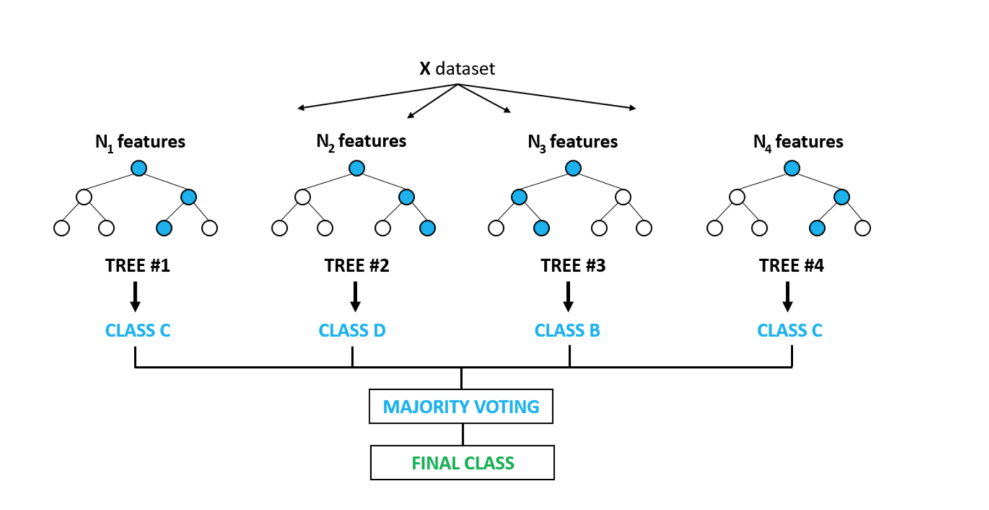
\includegraphics[width=\textwidth]{random-forest}}
    \caption{A Random Forest classification example (Copied from \cite{kirasich2018random})}
    \label{fig:rf}
\end{figure}

In the figure \ref{fig:rf}, the prediction through majority voting is \emph{class C}.
The main benefit purported by Random Forest algorithms include reduced risk of \gls{over-fitting} \cite{ibm:rf} and
resistance to redundant variables \cite{kirasich2018random};
however, they tend to be complex in terms of interpretability \cite{ibm:rf}.

\subsection{Multi-layer Perceptron}

Finally, a \gls{mlp} is a type of \gls{ann} with a feedforward mechanism (outputs are forwarded to the next layer) characterized by
an architecture that consists of an input layer, hidden layer(s), and an output layer;
it additionally makes use of backpropagation to adjust the weights of neurons to minimize the cost function of the output(s). \cite{taud2018multilayer}.


An example of a \gls{mlp} \gls{ann} can be seen in figure \ref{fig:mlp}  with three neurons in the input layer, two neurons in one hidden layer, and one neuron in the output layer.

\begin{figure}[H]
    \centering
    \AltText{A neural network showing neurons that are circular-shaped connected to other neurons in the next layer from left to right}{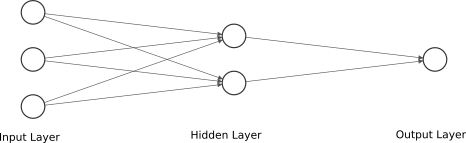
\includegraphics[width=\textwidth]{mlp}}
    \caption{A simple \gls{mlp} \gls{ann} with one hidden layer}
    \label{fig:mlp}
\end{figure}

In the figure \ref{fig:mlp}, the output of the two neurons in the hidden layer are a result of the application of an activation function.
Likewise the output of the neuron in the output layer is also activated---the activation functions used need not be the same in different layers.
Factors such as the number of hidden layers, number of iterations (steps to reduce the cost function), momentum and learning rate have an effect on the performance of a \gls{mlp} model \cite{taud2018multilayer}.

\clearpage%if the chapter heading starts close to bottom of the page, force a line break and remove the vertical vspace
\vspace{21.5pt}
\chapter{Implementation}\label{ch:proposed-solution}

The following sections detail the implemented solution to flag network traffic as malicious or benign.
The criteria for selecting tools used in the implementation was that they be freely available and open-source.
The implemented solution was divided into two separate parts, namely the network environment setup and model training parts.

The network environment setup dealt with generating malicious and benign traffic in a virtualized environment to be used later in testing the prediction of the models trained.
This part was not strictly necessary as traffic can be generated and captured in any network environment;
the rationale of creating such an environment was to capture only needed traffic in a safe environment, to keep the size of
capture packets small, and to increase privacy as captured packets might contain other network data when capturing in \gls{pr-mode}.

The model training part was concerned with creating machine learning models to analyze and flag the captured traffic in the virtual network.
Additionally, it also dealt with choosing the dataset used in training the models and other details involved in the whole process.


\section{Network Environment Setup}\label{sec:environment-setup}
The virtualized network environment was created with the help of \emph{Vagrant};
\emph{Vagrant} is a tool that can be used to quickly provision virtual machines.
The environment created with \emph{Vagrant} consisted of three machines all in the same network for simplicity since the aim was to generate and capture traffic.
All machines were created using a base image of Kali Linux, which is a popular OS used commonly in security testing scenarios.
The names and roles were assigned were as follows:

\begin{itemize}
    \item \emph{defender}: to capture traffic in the network
    \item \emph{attacker}: to generate malicious traffic
    \item \emph{target}: to act as a vulnerable server that can be attacked.
\end{itemize}

The \emph{target} machine had a version of \gls{dvwa} running on it.
\gls{dvwa} is an intentionally insecure web application which makes it a good candidate for testing malicious attacks.
The vulnerabilities discussed in chapter ~\ref{sec:malicious-network-traffic} are all possible in \gls{dvwa}.

\begin{code}
    \begin{minted}{ruby}
  config.vm.define "vulnerable-target" do |target|
    target.vm.hostname = "target"
    target.vm.network "private_network", ip: "192.168.60.60"
    target.vm.provider :virtualbox do |vb|
      vb.gui = false
      vb.name = "target"
      vb.memory = 1024
      vb.cpus = 1
    end
    target.vm.provision "bootstrap", type: "shell", path: "./make_dvwa_accessible_to_lan.sh", run: "once"
    target.vm.provision "start-dvwa", type: "shell", inline: "sudo dvwa-start", run: "always"
  end
    \end{minted}
\captionof{listing}{Provisioning the \emph{target} machine with \emph{Vagrant}}
\label{code:vagrant-target-provision}
\end{code}

The listing \ref{code:vagrant-target-provision} shows the code used in creating the \emph{target} machine.
While it is possible to use other providers, \emph{Virtualbox} was chosen because it had support in \emph{Vagrant} to modify
network device settings which was needed to set \gls{pr-mode} in the \emph{defender} machine.


With the virtual \gls{lan} created, the network traffic was generated in both malicious and benign stages.
In the malicious stage, the \emph{attacker} generated traffic for \gls{DoS}, \gls{sql} injection, command injection, brute force, and \gls{xss} attacks.
The \emph{attacker} machine in figure \ref{fig:attacker-box} shows how malicious network traffic was generated in the case of \gls{sql} injection that was aimed at the \emph{target} machine.

\begin{figure}[H]
    \centering
    \AltText{A view of the attacker machine OS interface showing a terminal client in the left-hand side and a web browser in the right-hand side}{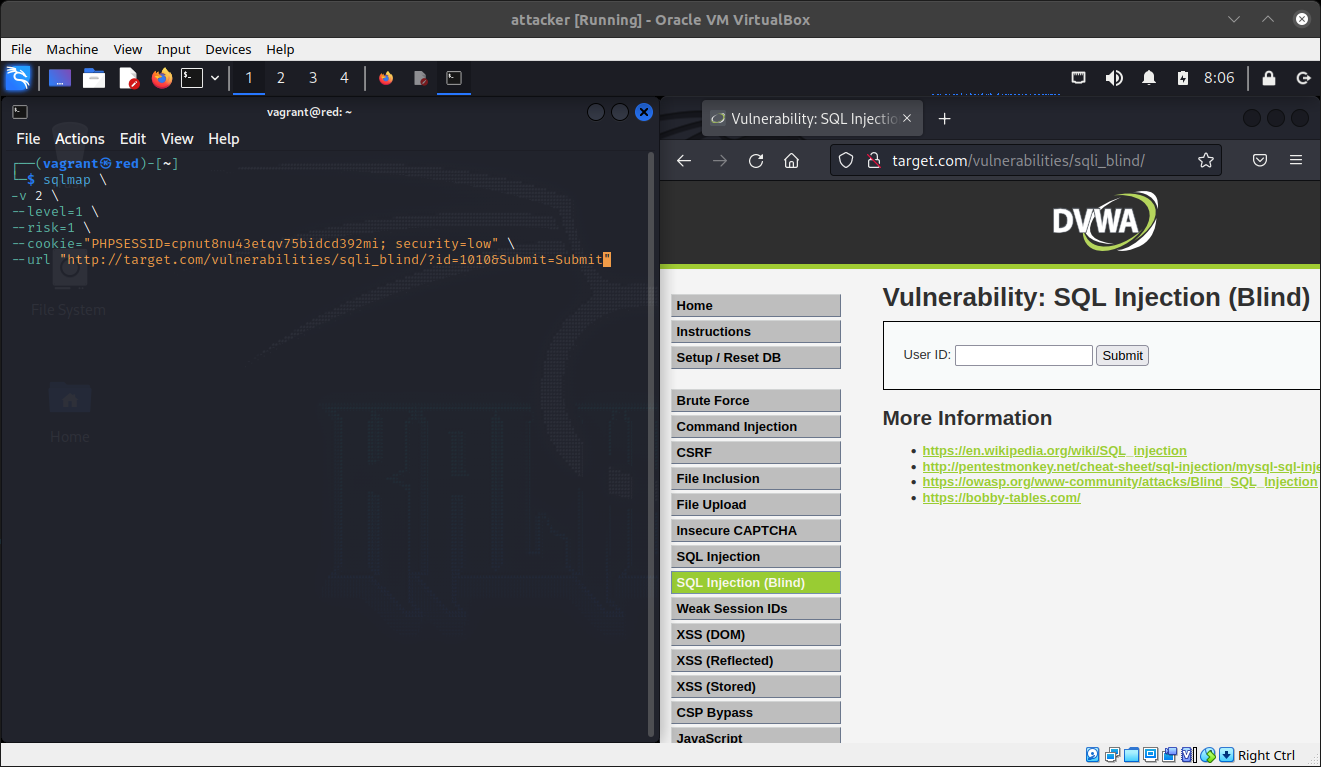
\includegraphics[width=\textwidth]{attacker-view}}
    \caption{Screenshot of \emph{attacker} machine preparing an \gls{sql} injection test}
    \label{fig:attacker-box}
\end{figure}


The figure \ref{fig:attacker-box} shows in view the web application to be attacked and the program \emph{sqlmap} to automate discovery of \gls{sql} vulnerabilities.
In contrast to the malicious stage which consisted only of traffic captured in the virtual \gls{lan},
the benign stage consisted of both virtual \gls{lan} and internet directed traffic.
The benign traffic consisted of web browsing of the \emph{target} machine's web application via \gls{http} without any attacks.
The rest of the benign traffic consisted of Telnet, \gls{dns}, \gls{ssh}, and \gls{ftp} protocol-related traffic.
Each scenario of the malicious and benign stages was captured in \gls{pcap} file format by the \emph{defender} machine using \emph{tcpdump}.
As a final step, the benign \gls{pcap} files were renamed to include the word `benign' in the filename to distinguish them from the malicious captures.


\section{Model Training}\label{sec:model-training}

This section focuses on the model training process and how it was implemented with machine learning methods:
\gls{knn}, Logistic Regression, \gls{mlp}, and Random Forest.
Training the models involved feeding them with labeled data to learn the patterns and relationships within the data.
The training was performed on a laptop with an `AMD® Ryzen 7 PRO 4750U' processor and 30.6 GiB of SODIMM DDR4 memory.

\subsection{Dataset}
The training process for classification tasks needs labeled data for supervised machine learning.
The quality, quantity, and representativeness of the dataset used can greatly impact the performance of the trained models.
It was deemed that the labeled data should contain at least some features that can be extracted (\gls{feat-extr}) easily from \gls{pcap} files.


The dataset eventually selected for use was the CICIDS2017 intrusion detection evaluation dataset \cite{sharafaldin2018toward}.
A newer version did exist at the start of the implementation (CSE-CIC-IDS2018), nonetheless CICIDS2017 was used due to its relative small size (under 900 MB).
The CICIDS2017 dataset with labeled data existed in CSV file format, those were downloaded and used in the model training.
Figure \ref{fig:dataset-label-dist} visually shows the composition of the CICIDS2017 dataset.

\begin{figure}[ht]
    \centering
    \AltText{A bar plot showing the distribution of labels in dataset with y-axis showing label count in logarithmic scale and x-axis showing the name of the attack label}{\includesvg[width=\textwidth]{dataset_label_distribution}}
    \caption{Dataset label distribution}
    \label{fig:dataset-label-dist}
\end{figure}

\clearpage
The dataset label distribution can be observed in figure \ref{fig:dataset-label-dist} showing the proportion of malicious labels to benign labels.
Due to the proportion of benign labels being higher in comparison to malicious labels (2,271,320 versus 556,556), one CSV file from the dataset (\texttt{\detokenize{Monday-WorkingHours.pcap_ISCX.csv}}) was dropped from the training process since it contained only benign labels.
The dataset was further preprocessed by removing identified redundant columns and one duplicate column;
moreover rows with infinity numbers were removed the dataset.
Finally, the columns with malicious labels were converted to the class number one while
benign labels were converted to the class number zero to make the training process straight-forward.
In the end the combined dataset after preprocessing had 2,298,395 rows with 71 columns where seventy columns were for features and one column for labels.


\subsection{Training Process}
The model training part as stated previously involves finding patterns within the dataset to make predictions for whether a particular piece of network traffic is malicious.
In the implementation of this stage, the \emph{scikit-learn} \cite{scikit-learn} library was chosen due to the availability of documentation and examples;
another reason was that it did not have any dependencies to GPU libraries, making it easy to install on different OS platforms.
The use of a machine learning library significantly reduced the implementation time since no time would be spent on algorithm coding.
The steps involved in the training process consisted of:

\begin{itemize}
    \item Creating the model pipeline.
    \item Training and tuning of \gls{hyper-param}.
    \item Cross-validation of models.
    \item Saving models in a persistent format.
\end{itemize}

The model pipeline is a list of steps that are chained together and can be applied to a piece of data input.
Listing \ref{code:knn-pipe} shows a \gls{knn} model pipeline as used in the training process implementation.
\clearpage

\begin{code}
    \begin{minted}{python}
def knn_model() -> Pipeline:
    return make_pipeline(
        StandardScaler(),
        LinearDiscriminantAnalysis(),
        KNeighborsClassifier(
            n_neighbors=3,
            p=2,
        ),
        verbose=True,
    )
    \end{minted}
\captionof{listing}{Setup of \gls{knn} pipeline}
\label{code:knn-pipe}
\end{code}

The pipeline shown in listing \ref{code:knn-pipe} contains three steps: scaling, dimensionality reduction, and the K-neighbors classifier itself.
The scaling of features step is an additional preprocessing step which depending on the learning algorithm itself might be needed or not;
in addition, the dimensionality reduction step helps reduce computation time---here it reduces the data dimensions from 70 to 1.
The last step in the pipeline is the \gls{knn} classifier with $K=3$ and $p=2$ to use the Euclidean distance metric (see chapter \ref{knn:theory}).
Contrast the parameters in listing \ref{code:knn-pipe} with listing \ref{code:rf-pipe}.

\begin{code}
\begin{minted}{python}
    return make_pipeline(
        RandomForestClassifier(
            n_estimators=100,
            criterion="gini",
            max_depth=None,
            max_features=35,
            min_samples_split=2,
            min_samples_leaf=2,
            bootstrap=False,
            max_samples=None,
            random_state=SEED,
            verbose=1,
            class_weight="balanced",
        ),
        verbose=True,
    )
\end{minted}
\captionof{listing}{Setup of Random Forest pipeline}
\label{code:rf-pipe}
\end{code}

\clearpage
As can be noted in listing \ref{code:rf-pipe}, some models can have more tunable \gls{hyper-param}.
Another difference that can be observed is that Random Forest does not need feature scaling since the algorithm is not sensitive to unscaled features.
Furthermore, the pipeline contains only one step so essentially the classifier can be used directly without including it in a pipeline;
the reason it was included is to make it easily comparable to the other models and additionally for code type checking.

The training part is straight-forward, the dataset is split into \gls{train-data} and \gls{test-data},
the portion of the \gls{test-data} was chosen to be a third of the dataset.
Each time the model pipeline was ran, the test score (calculated on the \gls{test-data}) and time taken was noted.
By tuning the \gls{hyper-param}, varying test scores could be observed;
in this way, a specific model's \gls{hyper-param} that perform best were eventually used.
Note that, the \gls{hyper-param} that had good performance where not necessarily used in the final training,
the time to train the model was also taken into account.
Therefore a balance between the two was the deciding factor on which \gls{hyper-param} were used.
For training the final models with the parameters chosen---the whole dataset is used, there was no need to set aside \gls{train-data}.

Be aware that there exist software libraries to automate the tuning of \gls{hyper-param} to find the best performing parameters or even the best predictive model itself.
This path was abandoned after a few rounds due to unreliability problems where the process would crash after a few days of training.

Additionally, \gls{cv} of the models was performed.
This was done to ensure that the models were not \gls{over-fitting} on the \gls{train-data}.
The \gls{cv} strategy chosen was a stratified k-fold wherein the \gls{train-data} was split into five folds and
the test score accuracy was compared.
A stratified strategy in the \gls{cv} was crucial since the dataset labels were not in equal proportions (see figure \ref{fig:dataset-label-dist}).

\clearpage
The last step in the training process was saving the models trained.
The importance of this step is that there is no need to train the model again in order to use it in network traffic prediction---this saves time and computation resources.
The other rationale is if sharing of the model is needed later.
There exist several formats for saving models, each with their advantage and disadvantages, for this implementation, the \emph{skops} library was chosen.
The main reason \emph{skops} was chosen is that it was created to work with the \emph{scikit-learn} library which made it easy to integrate within the project.
One disadvantage however with \emph{skops} is that the models trained cannot be imported in other programming languages,
therefore the saved models can only work with the specific version of Python programming language and \emph{scikit-learn} library used in the training process.

\subsection{Prediction Process}
Before the prediction based on the saved models was done, the \gls{pcap} files were first converted to CSV files;
this was done with the help of a software project called \emph{cicflowmeter}.
The version available at the time the project started was forked and modified to fix some errors and consequently included in this project
to do the conversion part.
The importance of the conversion from \gls{pcap} to CSV is that \gls{feat-extr} is performed on the network traffic data.
The \gls{feat-extr} process itself is out of scope of this thesis.
However, it suffices to say that \emph{cicflowmeter} (Python implementation) is based on \emph{CICFlowMeter} which is a Java software associated with the CICIDS2017 dataset used for feature extraction, among its other uses.


The prediction process in the implementation consisted of predicting the collected network traffic from the \gls{lan}.
For quick predictions, a \gls{gui} was created to facilitate this process as show in figure \ref{fig:gui}.


\begin{figure}[H]
\centering
\AltText{A GUI that shows three buttons, one for selecting the model, second for selecting the PCAP file and the third for predicting whether it is malicious or benign}{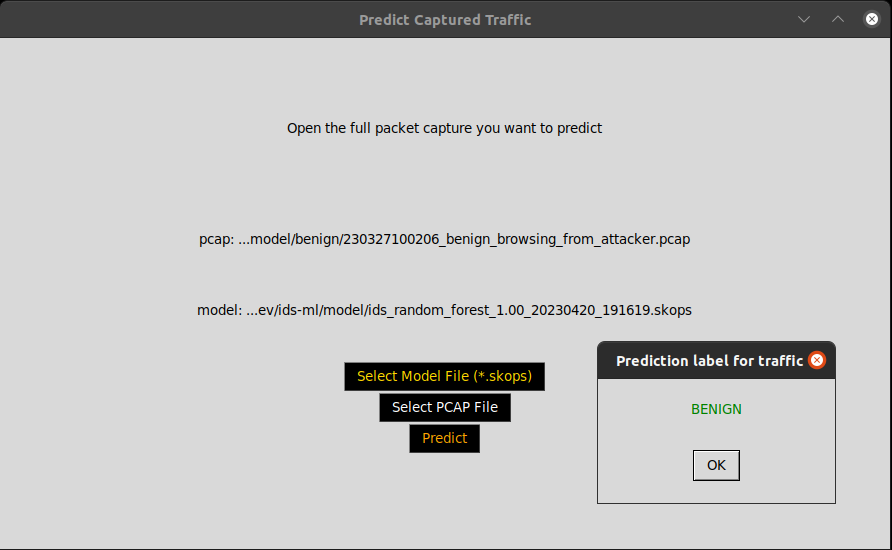
\includegraphics[width=\textwidth]{gui}}
\caption{Screenshot of the simple prediction \gls{gui}}
\label{fig:gui}
\end{figure}

The \gls{gui} in figure \ref{fig:gui} was created through Python's interface to the Tcl/Tk \gls{gui} toolkit called \emph{tkinter}.
The choice for using \emph{tkinter} instead of other more newer \gls{gui} toolkits, for instance, the \emph{Qt} framework, was
simply because the functionality desired was basic, namely, a few buttons, and a way to open files.

Through testing prediction of different models over time, it became cumbersome to observe and record predictions in this way.
As an alternative, a script to run predictions of different models on multiple \gls{pcap} files was implemented;
the script was meant to create a simple report showing how correct the predictions were in reality.
Figure \ref{fig:t-report} shows how the report looked in practice.


\begin{figure}[H]
\centering
\AltText{A text file showing the predictions for two models. It also show a summary of how many predictions were true and false}{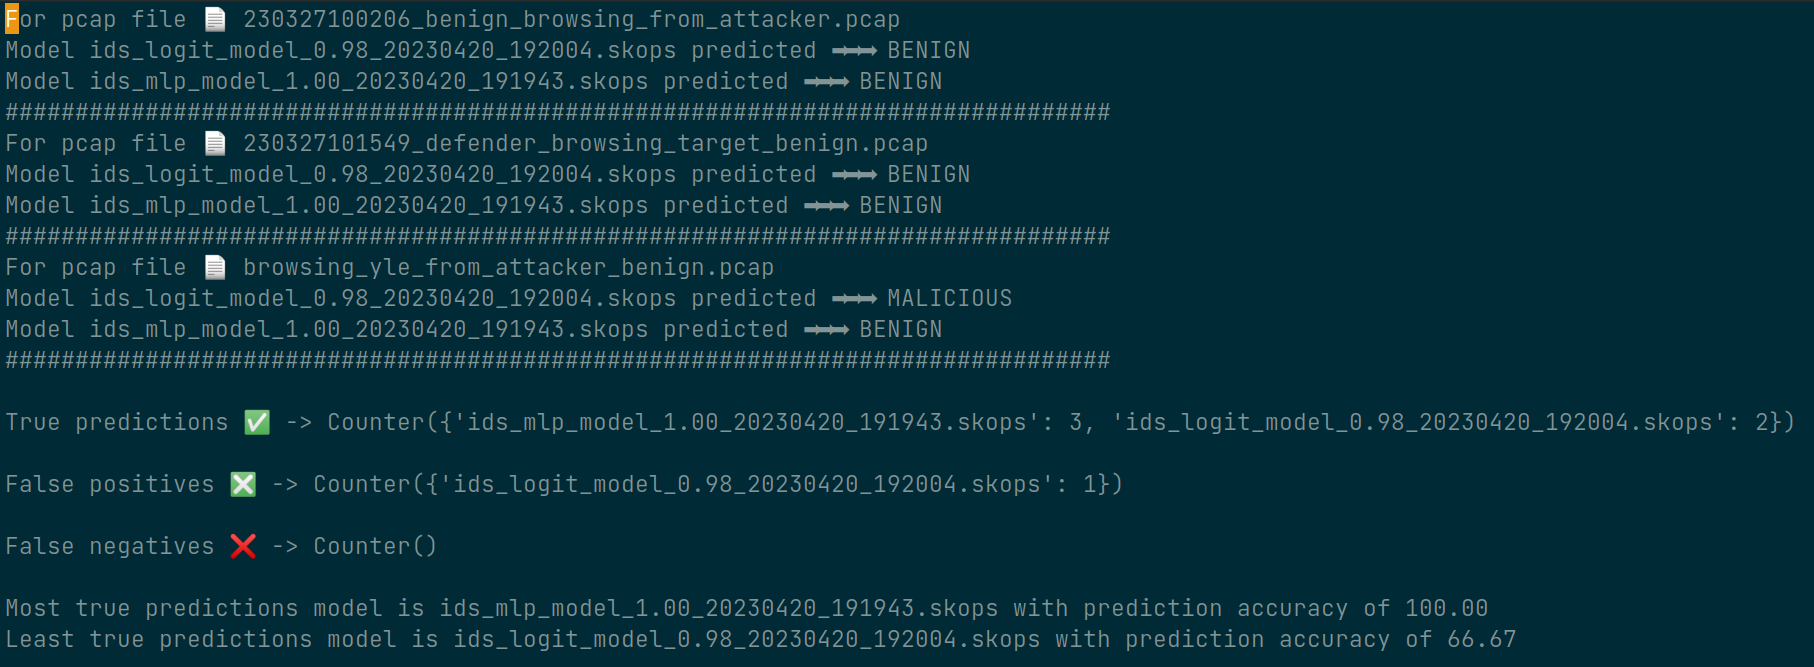
\includegraphics[width=\textwidth]{comparison-report}}
\caption{Screenshot of the simple report content}
\label{fig:t-report}
\end{figure}

The figure \ref{fig:t-report} also shows that the simple report created by the script details the count of true predictions, \gls{false-positive}s and \gls{false-negative}s.
Both the \gls{gui} and the script methods were used in different scenarios depending on what effort was required in regards to whether a single prediction was desired or multiple.

The full source code for the solution implementation can be found at \href{https://github.com/nicolaskyejo/ids-ml-exploration}{https://github.com/nicolaskyejo/ids-ml-exploration},
it contains both the network environment setup and the model \gls{hyper-param} used for the results obtained in the following chapter.

\clearpage%if the chapter heading starts close to bottom of the page, force a line break and remove the vertical vspace
\vspace{21.5pt}


\chapter{Results}\label{ch:results}

This chapter provides an evaluation of the models in terms of performance and the prediction results obtained.
The first section, Model Performance, describes the accuracy of the models and their ability to generalize to unseen data.
It compares and analyzes the respective performance on the CICIDS2017 dataset.
The second section, Prediction Results, presents the results of applying the models to data that was gathered from the implemented \gls{lan}.
It provides an analysis of the predictions made by the models, including the accuracy and reliability of the results.
Overall, this chapter provides insights into the performance and effectiveness of the models trained.

Recall, precision, and F1-score are evaluation metrics commonly used in binary classification tasks.
Recall measures the proportion of actual positive samples that are correctly identified as positive by the model
while
precision measures the proportion of predicted positive samples that are actually positive.
F1-score is the harmonic mean of recall and precision, which takes both metrics into account and provides an evaluation of a model's performance.
The F1-score ranges from zero to one, where one represents perfect precision and recall, and zero represents the worst performance.
The formula~\ref{eq:f1-equation} shows the calculation of the F1-score.

\begin{equation}
    \text{F1} = 2 \cdot \frac{\text{precision} \cdot \text{recall}}{\text{precision} + \text{recall}}\label{eq:f1-equation}
\end{equation}

where precision and recall are:

\begin{equation}
    \text{precision} = \frac{TP}{TP+FP}\label{eq:f1-precision-equation}
\end{equation}

\begin{equation}
    \text{recall} = \frac{TP}{TP+FN}\label{eq:f1-recall-equation}
\end{equation}

In the formulas~\ref{eq:f1-precision-equation} and~\ref{eq:f1-recall-equation}, $TP$ represents the number of true positives,
$FP$ represents the number of \gls{false-positive}s, and $FN$ represents the number of \gls{false-negative}s.
True positive in the implemented system represents the case where the network traffic is malicious.
In the \emph{scikit-learn} library, scores are calculated by passing the score metric that is desired and it will be calculated automatically.
These metrics are essential in evaluating the performance of a binary classification model and can help identify the strengths and weaknesses of the model in distinguishing between the two classes.


\section{Model Performance}\label{sec:model-performance}

The evaluation of a model's base performance was calculated on the basis of the dataset, whereas the collected network traffic was used in the final prediction.
For each model, different evaluations were done and recorded.
In this section, these evaluations are compared with each other.

One of the most important predictors of a model's performance is the learning curve.
A learning curve is a graphical representation that illustrates the progress of a model's learning by plotting its accuracy on the \gls{train-data} and
\gls{test-data} against the number of training samples.
The graph in figure~\ref{fig:learning-curve} shows the learning curve of the chosen machine learning models which depicts this relationship.

\begin{figure}[H]
    \centering
    \AltText{Four plots in vertical orientation showing a line plot depicting how accuracy is affected by number of samples}{\includesvg[width=\textwidth]{learning-curve-more-data-points}}
    \caption{Learning curve of the models on the dataset}
    \label{fig:learning-curve}
\end{figure}

As shown in figure~\ref{fig:learning-curve}, the models have different curves signifying that each model improved at different rates when more training samples were added.
The training score evaluates how the models performed on the \gls{train-data}, in other words, how well it was able to generalize the relationship between the input and output when the answers were known.
All models improved with the addition of more samples in the training set up to a point---this point was somewhere at about 36\% of the whole dataset samples.
Also of note is how Random Forest had a plateau while the other models except \gls{knn} slightly degraded in test score accuracy after this point.
A slightly more numerical comparison can be seen in figure~\ref{fig:conf-matrix}.


\begin{figure}[ht]
    \centering
    \AltText{A two by two diagram showing a box with numbers inside. These numbers signify the comparison between the predictions and the actual values}{\includesvg[width=\textwidth]{conf-matrix}}
    \caption{Confusion matrix of the models}
    \label{fig:conf-matrix}
\end{figure}

The figure~\ref{fig:conf-matrix} shows the confusion matrix diagram.
The number of $TP$, $FP$, $FN$, and $TN$ can be gleamed from the matrix.
It can be seen that the Random Forest model had the highest true predictions and the Logistic Regression model the highest missed predictions.
A more intuitive comparison can be observed in figure~\ref{fig:score-comparison} showing the mean F1-score of five cross-validated scores.

\begin{figure}[ht]
    \centering
    \AltText{A horizontal bar plot showing each models score in comparison}{\includesvg[width=\textwidth]{model_test_score_comparison}}
    \caption{Mean F1-score of models}
    \label{fig:score-comparison}
\end{figure}


The information learned from figure~\ref{fig:score-comparison} is similar to figure~\ref{fig:conf-matrix}.
It can be seen clearly that Random Forest had the highest score and \gls{knn} the lowest.
An explanation of why \gls{knn} score is the lowest is that the F1-score does not take into account the number of $TN$.

Another useful comparison from the training process was how the models performed in terms of time taken to train;
this information can affect resource planning optimization when considered together with model accuracy.
This comparison can be seen in figure~\ref{fig:train-time}.

\begin{figure}[ht]
    \centering
    \AltText{A vertical bar plot where each bar represents each model's train time}{\includesvg[width=\textwidth]{model_training_time_comparison}}
    \caption{Model training time on full dataset}
    \label{fig:train-time}
\end{figure}

The training time shown in figure~\ref{fig:train-time} reveals that Random Forest took the longest time to train while
\gls{knn} the shortest.
In regards to \gls{knn}, the result is not surprising since the model's computation only takes place during prediction of new data.
The training process results show that all the models used can be justified as good models when their training time and F1-scores are examined together.


\section{Prediction Results}\label{sec:prediction-results}

In this section, the prediction results obtained from the trained models on the captured network data (\gls{pcap}) are discussed.
The prediction results are analyzed to evaluate the performance of each model in terms of precision, recall, and F1-score.
By comparing the results of different models, the most effective model for predicting network traffic can be identified.
Additionally, the potential implications of the prediction results are briefly addressed.
Table~\ref{tab:table-final-results} shows the predictions of the captured network traffic in the \gls{lan}.


\begin{table}[htbp]
    \centering
    \caption{Prediction results for different models on captured network data}
    \label{tab:table-final-results}
    \begin{tabular}{|l|l|l|l|l|l|}
        \hline
        \textbf{\gls{pcap} type}      & \textbf{Label} & \textbf{KNN} & \textbf{MLP} & \textbf{RF} & \textbf{LR} \\ \hline
        Web browsing on target        & Benign         & Benign       & Malicious    & Benign      & Benign                       \\ \hline
        Telnet connection             & Benign         & Benign       & Benign       & Benign      & Benign                       \\ \hline
        \gls{ftp} connection          & Benign         & Benign       & Benign       & Benign      & Benign                       \\ \hline
        \gls{ssh} connection          & Benign         & Benign       & Benign       & Benign      & Benign                       \\ \hline
        \gls{dns} query               & Benign         & Benign       & Benign       & Benign      & Benign                       \\ \hline
        %%%%%%%%%%%%%%%%%%%%%%%%%%%%%%%%%%%%%%%%%%%%%%%%%%%%%%%%%%%%%%%%%%%%%%%%%%%%%%%%%%%%%%%%%%%%%%%%%%%%%%%%%%%%%%%%%%%%%%%%%%%%%%%%%%%%%%%%%%%%%%%%%%%%%%%%%
        Brute force login             & Malicious      & Malicious    & Malicious    & Benign      & Benign                       \\ \hline
        \gls{DoS} by \gls{icmp} flood & Malicious      & Malicious    & Benign       & Benign      & Malicious                    \\ \hline
        \gls{sql} injection           & Malicious      & Malicious    & Malicious    & Benign      & Malicious                    \\ \hline
        Command injection             & Malicious      & Malicious    & Malicious    & Benign      & Malicious                    \\ \hline
        \gls{xss}                     & Malicious      & Benign       & Malicious    & Benign      & Benign                       \\ \hline
    \end{tabular}
\end{table}

From the data in table~\ref{tab:table-final-results}, the results suggest that \gls{knn} is the most accurate model.
The F1-scores (see formula~\ref{eq:f1-equation}) of \gls{knn}, \gls{mlp}, Random Forest, and Logistic Regression are 0.89, 0.80, 0.00, and 0.75 respectively.
The expectation from the final model performance is somewhat different---especially in regards to Random Forest and \gls{knn}.
One explanation could be that Random Forest was \gls{over-fitting} on the dataset and \gls{knn} model did not.
\gls{knn} as the most accurate model in the final results predicted everything correctly except the \gls{xss} attack;
\gls{mlp} \gls{ann} as the second most accurate model incorrectly flagged \gls{http} web browsing traffic as malicious and missed the \gls{DoS} attack.
The Logistic Regression model as the third most accurate model missed the brute force and \gls{xss} attacks.

\clearpage
According to the dataset publication, command injection attack was not part of the dataset.
Despite this, the models were able to correctly flag it as malicious (except Random Forest) which can be evidence of the power of \gls{aids} to detect new or unseen attacks.

However, it should be noted that to calculate a meaningful F1-score, more observation data is needed with varying attack and benign samples.
Therefore, the final results are only a suggestive result rather than a conclusive result.
In the end, a combination of \gls{aids} to detect \gls{zero-day} attacks and \gls{sids} to detect known attacks may be the most effective method in
forensics of malicious network traffic.

\clearpage%if the chapter heading starts close to bottom of the page, force a line break and remove the vertical vspace
\vspace{21.5pt}


\chapter{Conclusion}\label{ch:conclusions}

The primary goals of this thesis were to detect malicious network traffic,
investigate the practical implementation of a forensic system for this purpose,
and evaluate its effectiveness as a low-cost security solution.
Through the application of supervised machine learning methods,
it was demonstrated that it is possible to detect malicious traffic in a reliable way.

Regarding the practical implementation process, it was heavily reliant on the availability of open datasets.
Without available open datasets, the process would have been arduous.
The training process itself was fairly straight-forward with most time spent on tuning \gls{hyper-param}.
Therefore, the goal of practical implementation is indeed realistic to achieve when quality datasets are obtainable.

As to the effectiveness as a low-cost security solution,
it depends on the resources available to an individual or an organization.
For entities with considerable capital and resources,
it can be feasible to allocate some of those resources to train such network forensic models
and even create datasets that are used for that purpose.
However, in a market economy it can be seen as a waste of resources to do so,
therefore, it is more probable that a few organizations or companies sell their own solutions to others.
Nevertheless, it can be assumed that organizations with high-security profiles, for example,
government agencies and military facilities are creating
and using their own network forensic solutions which are considered as a low-cost security solution to them.

While this thesis has achieved its main goal, it is important to recognize some limitations as well.
One weakness is the limited the number of attack type scenarios that were examined,
both in the actual dataset and the ones generated for the final evaluation;
more attack data would have raised the confidence of the final results.
Another limitation is
that the trained models were not tested in a real-world network which could have brought interesting observations.

In closing,
one area of further research recommended is the development of open datasets
that can be used to create network forensic solutions.
Most of the current available datasets rely
on creating malicious traffic in a virtualized environment and labelling them appropriately;
this can be considered a cumbersome and time-consuming process.
It could be feasible to crowdsource the creation of such datasets with multiple organizations
contributing their traffic captures and logs.
The inherent privacy issues of such an approach could be alleviated with some form of anonymization techniques,
perhaps again with the help of machine learning methods.



%----------------------------------------------------------------------------------------
%	BIBLIOGRAPHY REFERENCES
%----------------------------------------------------------------------------------------

% Bibliography.
% Normally you do not edit this file.
% To add bibliography in your text, add them first in the biblio.bib file and
% reference them with the \cite{} command in your text. Check also \citeauthor
% and \citeyear (e.g. for copied figure caption), the \cites for multi-cites
% with page numbers,...

\clearpage
%line space
%\singlespacing %removed otherwise the appendix are also single space
\begin{singlespacing}
\vspace*{-16pt}
\printbibliography[title=\IfLanguageName{finnish}{Lähteet}{References}]
\end{singlespacing}

%for counting the pages
\label{LastPage}~


%----------------------------------------------------------------------------------------
%	APPENDICES
%----------------------------------------------------------------------------------------

%\input{style/appendix.tex}
%%force smaller vertical spacing in table of content
%%!!! There can be some fun depending if the appendices have (sub)sections or not :D
%% You will have to play with these numbers and eventually add the \vspace line  before
%% some \chapter and force another number.
%% To add more fun, time to time the table of content get wrong after a build :(
%\addtocontents{toc}{\vspace{11pt}}
%\pretocmd{\chapter}{\addtocontents{toc}{\protect\vspace{-24pt}}}{}{}

%\liite{1}% This is a hack to have right page numbering for each appendix. Make sure to
% use a unique number for each appendix.
%\input{sample/Xappendix1.tex}% Sample content to demonstrate appendix in LaTeX. You
% are safe to delete this lines (and the next samples) once you refreshed your LaTeX
% skills (and safe to delete the sample folder and all its file too).

%\addtocontents{toc}{\vspace{11pt}}%fix vertical space for Table of Content
%\liite{2}
%\input{sample/Xappendix2.tex}
%
%\addtocontents{toc}{\vspace{11pt}}
%\liite{3}
%\input{sample/X_R_example.tex}


%----------------------------------------------------------------------------------------
%	THIS IS THE END
%----------------------------------------------------------------------------------------
\end{document}
